\section{Các công trình nghiên cứu có liên quan}\label{sec:intro}
\frame{\tableofcontents[currentsection]}

\subsection{Lip Movements Generation at a Glance\cite{chen2018}}
\begin{frame}{Lip Movements Generation at a Glance}
    \begin{figure}[H]
    \centering
    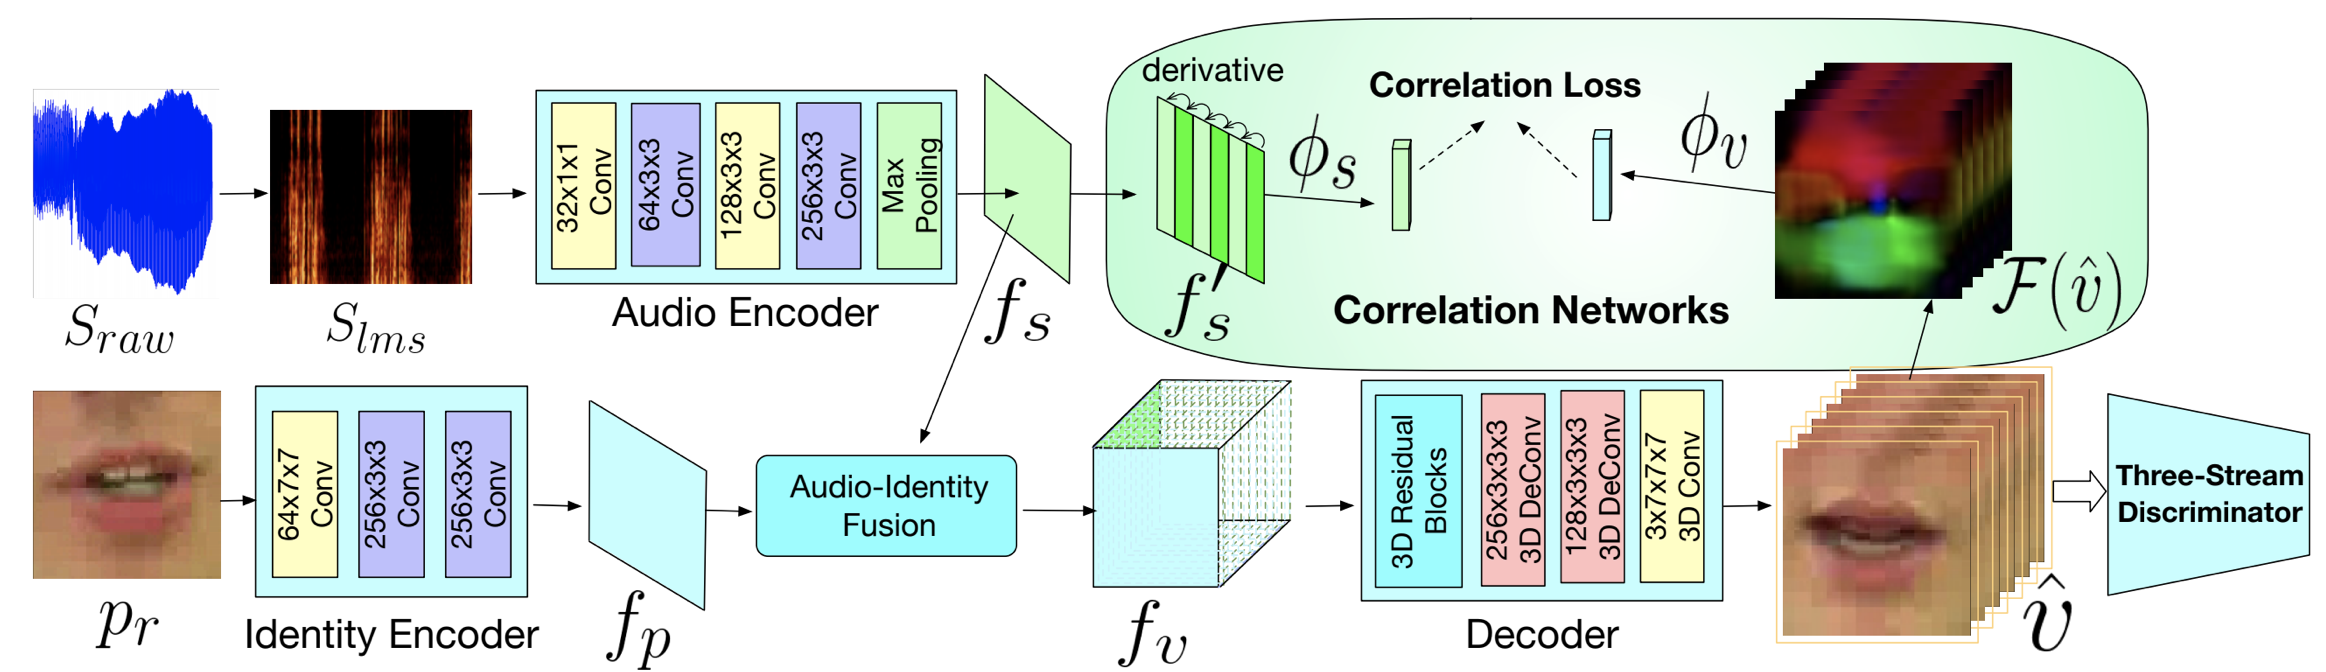
\includegraphics[width=12cm]{images/chen2018_model.png}
    \label{fig:chen2018_model}
    \caption{Kiến trúc mô hình}
    \end{figure}
\end{frame}

\begin{frame}{Lip Movements Generation at a Glance}
    \begin{figure}[H]
        \centering
        \begin{minipage}{0.48\textwidth}
            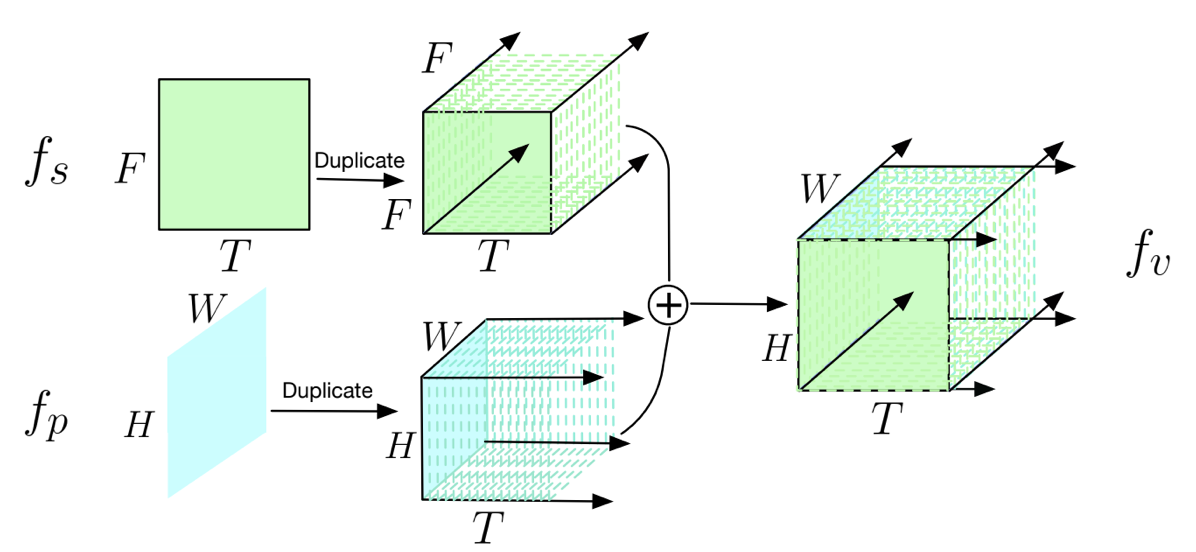
\includegraphics[width=7cm]{./images/chen2018_fusion.png}
            \caption{Phương pháp kết hợp đặc trưng hình ảnh và âm thanh}
            \label{fig:chen2018_fusion}
        \end{minipage}\hfill
        \begin{minipage}{0.48\textwidth}
            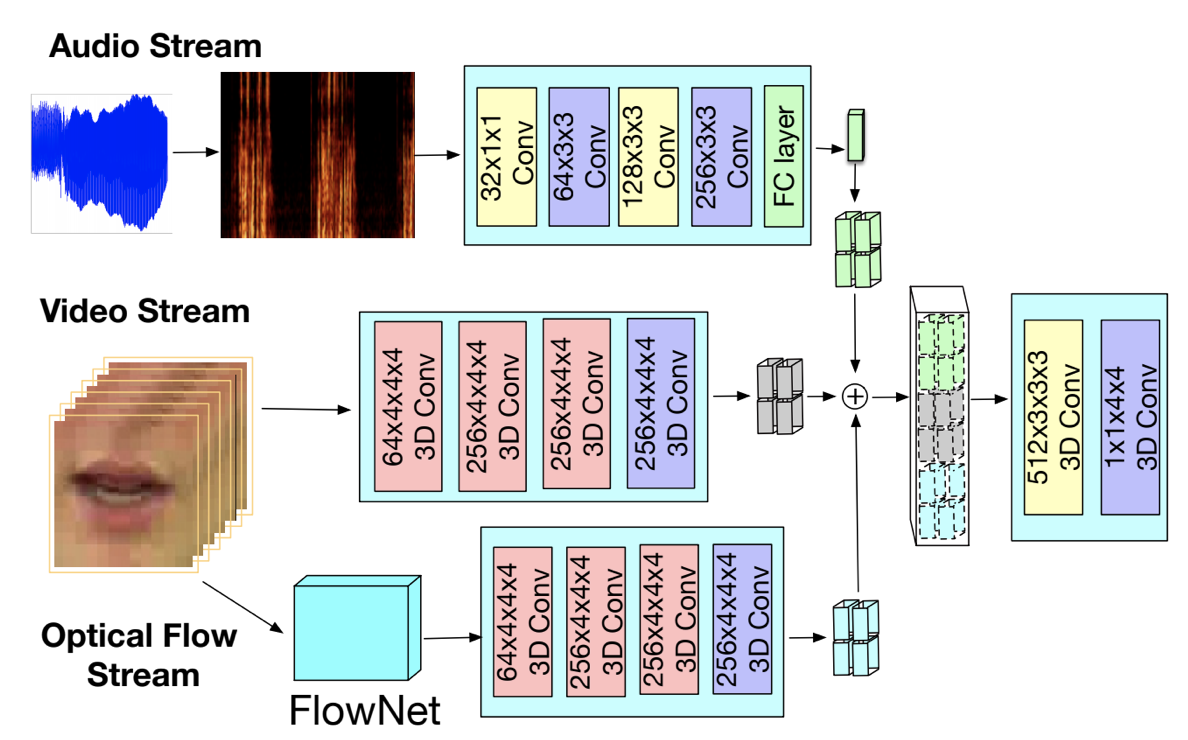
\includegraphics[width=7cm]{./images/chen2018_gans.png}
            \caption{GANs Discriminator với 3 loại đặc trưng}
            \label{fig:chen2018_gans}
        \end{minipage}
    \end{figure}
\end{frame}

\begin{frame}{Lip Movements Generation at a Glance}
    \begin{itemize}
        \item Ưu điểm
        \begin{itemize}
            \item Đưa ra các phương pháp phù hợp và tiến bộ để trích xuất và kết hợp đặc trưng hình ảnh và âm thanh
            \item Tận dụng phương pháp GANs để cải thiện chất lượng của ảnh
            được tạo sinh
        \end{itemize}
        \item Khuyết điểm
        \begin{itemize}
            \item Mạng chỉ có thể nhận vào hình ảnh tĩnh và một đoạn âm thanh có độ dài xác định (0.64s) và cho ra số khung hình tương ứng với khoảng thời gian đó (16 khung hình)
            \item Chưa chú ý đến hiện tượng nhảy hình của video được tạo sinh, mạng không có cơ chế để đảm bảo việc chuyển ảnh mượt mà, ít sai khác về độ tương phản, ánh sáng, màu sắc giữa các khung ảnh gần nhau
        \end{itemize}
    \end{itemize}
\end{frame}

\subsection{Realistic Speech-Driven Facial Animation with GANs\cite{vougioukas2020}}
\begin{frame}{Realistic Speech-Driven Facial Animation with GANs}
    \begin{figure}[H]
        \centering
        \begin{minipage}{0.48\textwidth}
            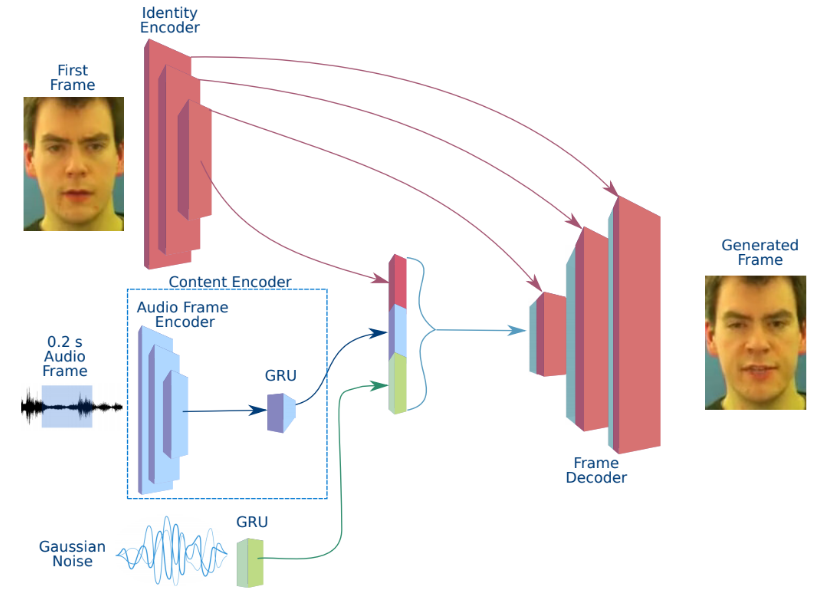
\includegraphics[width=7cm]{./images/vou2020_generator.png}
            \caption{Bộ Generator}
            \label{fig:vou2020_generator}
        \end{minipage}\hfill
        \begin{minipage}{0.48\textwidth}
            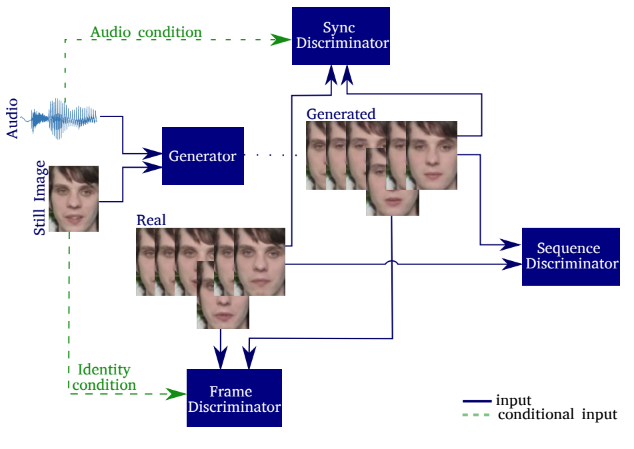
\includegraphics[width=7cm]{./images/vou2020_model.png}
            \caption{GANs Discriminator với 3 đặc trưng}
            \label{fig:vou2020_model}
        \end{minipage}
    \end{figure}
\end{frame}

\begin{frame}{Realistic Speech-Driven Facial Animation with GANs}
    \begin{figure}[H]
        \centering
        \begin{minipage}{0.48\textwidth}
            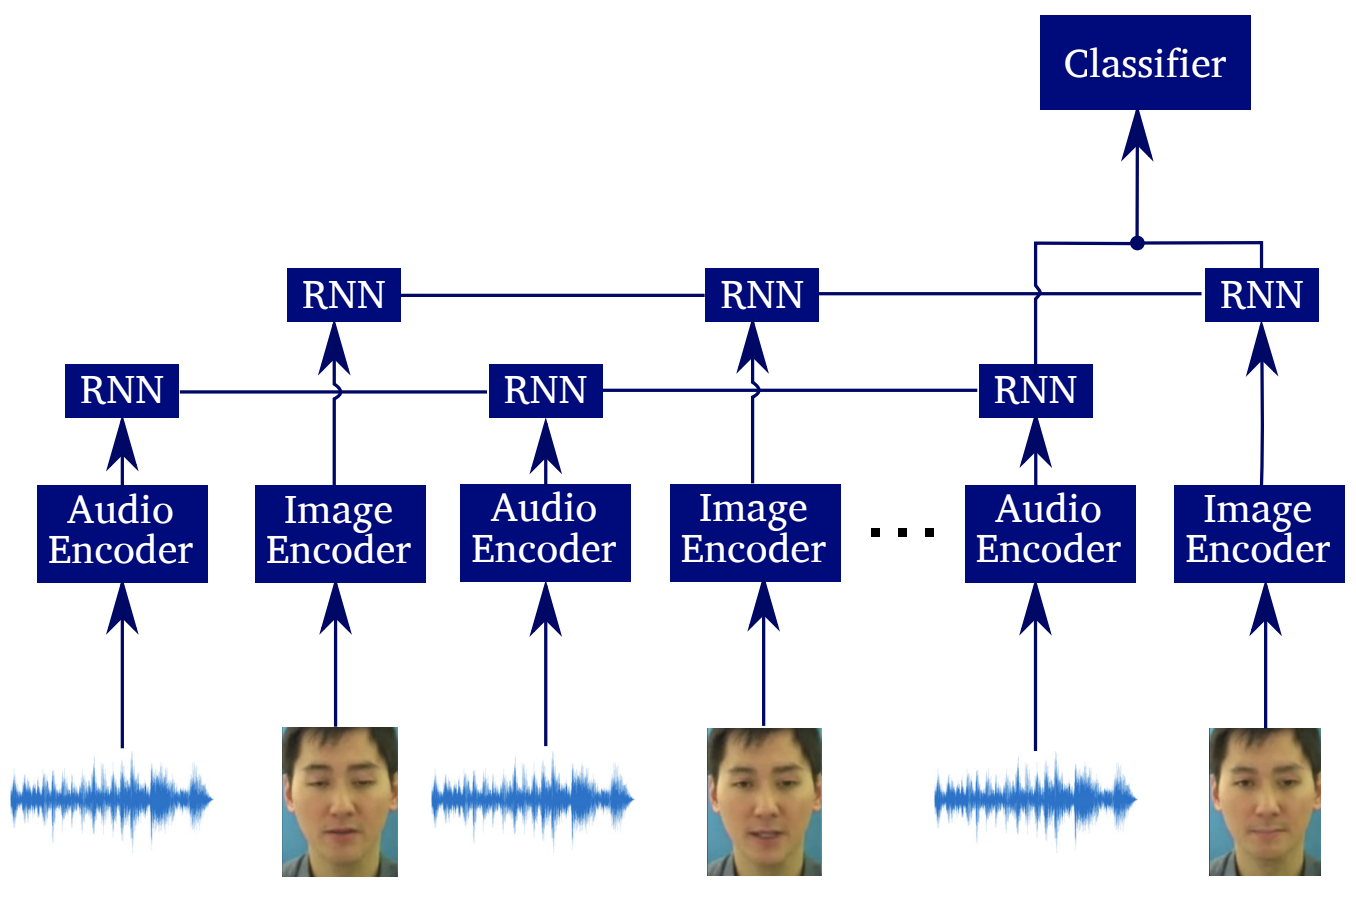
\includegraphics[width=7cm]{./images/vou2019_seq_dis.png}
            \caption{Sequence Discriminator}
            \label{fig:vou2020_generator}
        \end{minipage}\hfill
        \begin{minipage}{0.48\textwidth}
            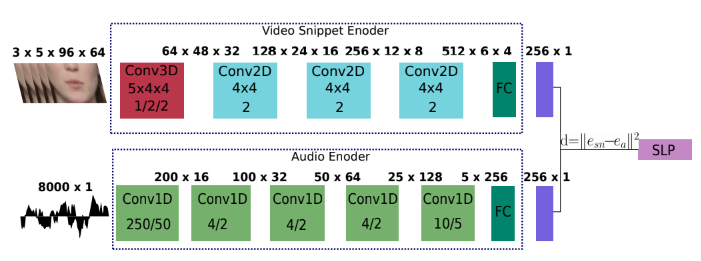
\includegraphics[width=7cm]{./images/vou2020_sync_dis.png}
            \caption{Sync Discriminator - Ba trường hợp: ảnh-âm gốc, ảnh-âm lệch, ảnh tạo sinh - âm}
            \label{fig:vou2020_model}
        \end{minipage}
    \end{figure}
\end{frame}

\begin{frame}{Realistic Speech-Driven Facial Animation with GANs}
    \begin{itemize}
        \item Ưu điểm
        \begin{itemize}
            \item Đưa ra các phương pháp tạo sinh khuôn mặt có chú ý đến khẩu hình miệng và sự mượt mà trong chuyển động giữa các khung hình
            \item Dùng xác suất ngẫu nhiên để sinh ra chuyển động ở các vị trí khác trên mặt (mắt)
            \item Hạn chế việc lệch tiếng nói nhờ Sync Discriminator
        \end{itemize}
        \item Khuyết điểm
        \begin{itemize}
            \item Chưa thể hiện được các biểu cảm trên gương mặt
            \item Chưa chú ý đến chuyển động của đầu
            \item Chưa chú trọng việc tái tạo môi trường xung quanh
            \item Không tái tạo tốt đặc điểm gương mặt của những người không nằm trong tập huấn luyện
        \end{itemize}
    \end{itemize}
\end{frame}
